
\subsection{Benchmarking DBMS}

One of the harder aspects of data management is the performance analysis and tuning. For complex systems that perform high workloads on large datasets, it is particularly challenging because many factors can affect the performance. In terms of \gls{dbms}, this is done by the usage of a benchmark that allows one to evaluate the system's main performance metrics under stressful conditions \cite{10.14778/2732240.2732246}.


Benchmarks are techniques that seek to collect and compare a wide variety of activities, to achieve the best result, an objective criterion for determining which practice or software is superior in certain scenarios that the user who
is doing the simulation built. An example of popular questions is "Which domain is the best system?”. The SPECCpu benchmark ~\cite{henning2006spec}, for instance, addresses the question, "What is the best \gls{cpu}?" "and the \gls{tpcc} ~\cite{council2010tpc} responds to the question, "What is the best \gls{oltp} database system?” ~\cite{benchmarkchen,benchcloud}.

For \citeauthor{gray1992benchmark}, a domain-specific benchmark must meet four criteria to be an effective benchmark. It must be:

\begin{itemize}
    \item \textbf{Relevant:} In performing typical operations within that problem domain, it must measure the peak performance and price/performance of systems. 
    \item \textbf{Portable:} It should be easy to implement the benchmark on many different systems and architectures.
    \item \textbf{Scaleable:}  The benchmark should apply to computer systems small and large. As computer performance and architecture evolve, it should be possible to scale the benchmark up to bigger systems and to parallel computer systems.
    \item \textbf{Simple:} The benchmark must be understandable, otherwise credibility will be lacking.
\end{itemize}



%For conducting the measurements of the energy spent, we need first a benchmark tool that can be a load generator system that can emulate a real environment in \gls{dbms}.

\subsubsection{TPC Benchmark C}
\glsfirst{tpcc} is an \gls{oltp} workload~\cite{council2010tpc}. It is a mixture of read-only and update intensive transactions that simulate the activities found in complex \gls{oltp} application environments. It does so by exercising a breadth of system components associated with such environments, which are characterized by:

\begin{itemize}
    \item The simultaneous execution of multiple transaction types that span a breadth of complexity
    \item On-line and deferred transaction execution modes
    \item Multiple on-line terminal sessions
    \item Moderate system and application execution time
    \item Significant disk input/output
    \item Transaction integrity (\gls{acid} properties)
    \item Non-uniform distribution of data access through primary and secondary keys
    \item Databases consisting of many tables with a wide variety of sizes, attributes, and relationships
    \item Contention on data access and update
\end{itemize}

While these specifications express implementation in terms of the relational data model with a traditional locking framework, any commercially available \gls{dbms}, database servers, file systems, or other data repositories offering a functionally equivalent implementation can be used to implement the database.

\gls{tpcc} uses metrics and terminology that are similar to other benchmarks originating from the TPC or others. In no way does this similarity in terminology imply that the results of \gls{tpcc} are comparable to other benchmarks. Other \gls{tpcc} results compliant with the same revision are the only benchmark results comparable to \gls{tpcc}.

The performance metric reported by \gls{tpcc} is a "business throughput" measuring the number of orders processed per minute. Multiple transactions are used to simulate the business activity of processing an order, and each transaction is subject to a response time constraint. The performance metric for this benchmark is expressed in transactions per minute. 

\gls{tpcc} is accepted in the industry as the most credible transaction processing benchmark with a large body of results across all major hardware and database platforms. The highly tuned and optimized nature of the \gls{tpcc} configurations makes it the best candidate for study \gls{dbms} power consumption~\cite{powerconsumptiontppc}.

\subsubsection{HammerDB}
\label{sc:hammerdb}


 
HammerDB is an open source and widely used benchmark framework for the worlds most popular DBMS~\cite{scalzo2018database,elgrablyanalise,knoche2016combining,benchmarkchen,ali2019persistent,yu2015design,koccak2018software,koccak2018software}.   HammerDB emulates a \gls{tpcc} scenario  and through \gls{oltp} workloads it sets up a company's sales processing environment. It reduces the testing costs by simplifying the \gls{tpcc} rules, which can be modified and run on a custom environment. The above factors result in a low-cost solution, rapid deployment, and customized DBMS benchmark system~\cite{benchmarkchen,elgrablyanalise,hammerdb}. HammerDB currently supports Oracle, SQL Server, Db2, TimesTen, MySQL, MariaDB, PostgreSQL, Greenplum, Postgres Plus Advanced Server, and Redis. Moreover, it can run on a variety of operating systems, making it a  flexible and heterogeneous benchmarking framework~\cite{benchmarkchen}.


\begin{figure}[h!]
    \centering
    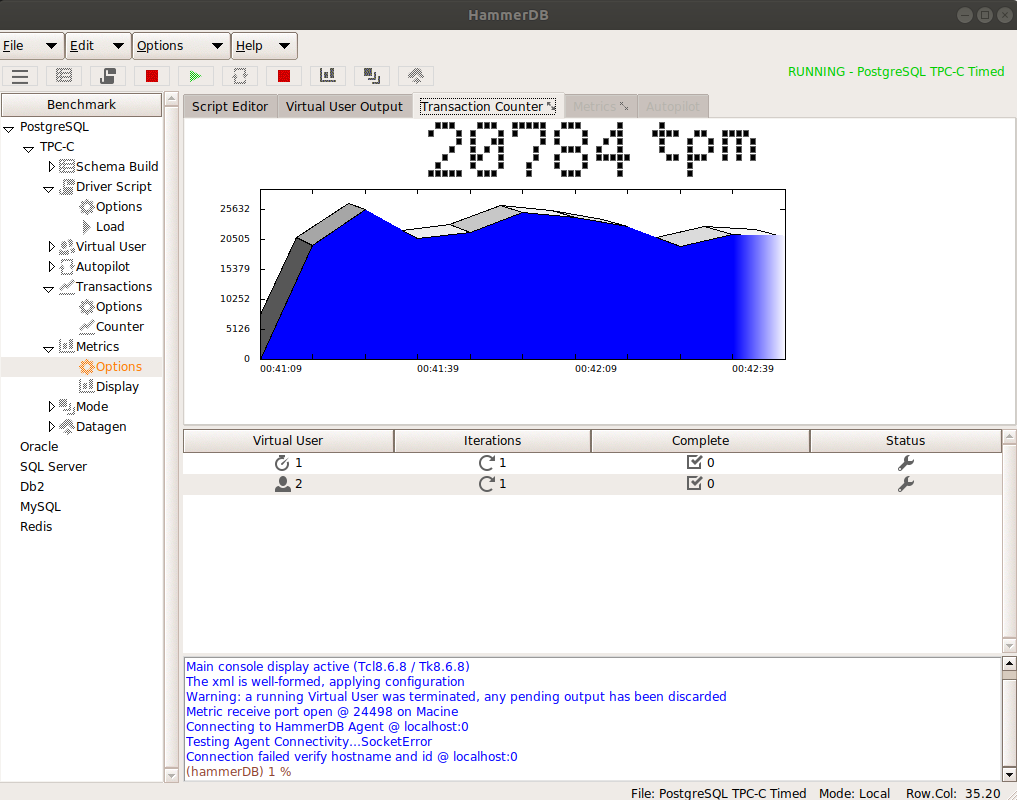
\includegraphics[width=0.6\columnwidth]{Chapters/images/hammerdb1.png}
        \caption{HammerDB GUI.}
    \label{fig:hamerdbgui}
    \end{figure}

Although HammerDB implements a workload based on the \gls{tpcc} specification, it does not implement a complete \gls{tpcc} benchmark specification. As a consequence,  the transaction results from HammerDB can not be compared  to the official \gls{tpcc} benchmarks. HammerDB workloads generate 2 statistics. \gls{tpm} is the transactional measurement of the specific database typically defined as the number of user commits plus the number of user rollbacks. \gls{tpm} values are database-specific and, thus, they cannot be compared among different DBMS. The \gls{nopm} value, on the other hand, is a performance metric independent of any particular database implementation and it is the recommended primary metric to use~\cite{hammerdb}.

%\discuss{Aqui tem vários screenshots do hammerDB que acho que fazia sentido teres um do género aqui:
%\url{https://www.hammerdb.com/about.html}}




HammerDB is being actively used by researchers to study the performance of DBMS: \citeauthor{elgrablyanalise} use HammerDB to compare open-source DBMS performance like Mysql, MariaDB and Postgres \cite{elgrablyanalise}. Another study that uses Hammerdb is \citeauthor{knoche2016combining}~(\citeyear{knoche2016combining}) work that uses HammerDB to test the impact of database lock contention in the \gls{tpcc} benchmark scenario~\cite{knoche2016combining}. In the context of green computing,  \citeauthor{koccak2018software}~(\citeyear{koccak2018software}) uses HammerDB with MySQL to define a dataset to use on his software energy consumption prediction~\cite{koccak2018software}. 

HammerDB is also being widely used by most leading database and technology companies, such as Oracle, IBM, Intel, Dell/EMC HPE, Huawei, Lenovo, and hundreds more~\cite{hammerdb}. . It has been downloaded hundreds of thousands of times in more than 180 countries.




%\discuss{Dizer isto no capitulo seeguinte: aqui apenas descreves o hamerdb. No capitulos eguinte é que justificas o porquês de o usar}

%We decide to use HammerDB as it is a benchmark tool that can replicate the behavior of most cloud-based applications as a service, verify comprehensive performance and multiple metrics in a simple real-world environment on a virtual environment with virtual users~\cite{hammerdb}.

%Another reason we choose him was that HammerDB is used for automated software testing~\cite{hammerdb} so we can configure how many times the HammerDB will run and how many virtual users that he will use and for how long it will run, providing at the end of every execution the \gls{tpm} and the \gls{nopm}. With these numbers and the energy spent, we can have ample information to answer the RQ2, and with an adjustable number of users, it can assist in the RQ3.

